% !TEX encoding = UTF-8 Unicode
%%%%%%%%%%%%%%%%%%%%%%%%%%%%%%%%%%%%%%%%%
% Journal Article
% LaTeX Template
% Version 1.4 (15/5/16)
%
% This template has been downloaded from:
% http://www.LaTeXTemplates.com
%
% Original author:
% Frits Wenneker (http://www.howtotex.com) with extensive modifications by
% Vel (vel@LaTeXTemplates.com)
%
% License:
% CC BY-NC-SA 3.0 (http://creativecommons.org/licenses/by-nc-sa/3.0/)
%
%%%%%%%%%%%%%%%%%%%%%%%%%%%%%%%%%%%%%%%%%

%----------------------------------------------------------------------------------------
%	PACKAGES AND OTHER DOCUMENT CONFIGURATIONS
%----------------------------------------------------------------------------------------
\documentclass[oneside, 11 pt]{article}
\usepackage[utf8]{inputenc}
\usepackage[T1]{fontenc}
\usepackage{textcomp}
\usepackage[portuguese]{babel}
\usepackage{blindtext} % Package to generate dummy text throughout this template 
\usepackage{comment}
\usepackage{listings}
\usepackage{xcolor}
\usepackage{hyperref} % For hyperlinks in the PDF

\usepackage{inconsolata}
\lstset{
	language=bash, %% Troque para PHP, C, Java, etc... bash é o padrão
	basicstyle=\ttfamily\small,
	numberstyle=\footnotesize,
	backgroundcolor=\color{gray!10},
	frame=single,
	tabsize=2,
	rulecolor=\color{black!30},
	escapeinside={\%*}{*)},
	breaklines=true,
	breakatwhitespace=true,
	framextopmargin=2pt,
	framexbottommargin=2pt,
	inputencoding=utf8,
	extendedchars=true,
	literate={á}{{\'a}}1 {ã}{{\~a}}1 {é}{{\'e}}1 {í}{{\'i}}1,
}
\usepackage[hmarginratio=1:1,top=32mm,columnsep=20pt]{geometry} % Document margins
\usepackage[hang, small,labelfont=bf,up,textfont=it,up]{caption} % Custom captions under/above floats in tables or figures
\usepackage{booktabs} % Horizontal rules in tables

\usepackage{lettrine} % The lettrine is the first enlarged letter at the beginning of the text

\usepackage{enumitem} % Customized lists
\setlist[itemize]{noitemsep} % Make itemize lists more compact

\usepackage{titlesec} % Allows customization of titles
%\renewcommand\thesection{\Roman{section}} % Roman numerals for the sections
%\renewcommand\thesubsection{\roman{subsection}} % roman numerals for subsections
\titleformat{\section}[block]{\large\scshape\centering}{\thesection.}{1em}{} % Change the look of the section titles
\titleformat{\subsection}[block]{\large}{\thesubsection.}{1em}{} % Change the look of the section titles

\usepackage{fancyhdr} % Headers and footers
\pagestyle{fancy} % All pages have headers and footers
\fancyhead{} % Blank out the default header
\fancyhead[C]{Tutorial do Bash} % Custom header text

\usepackage{titling} % Customizing the title section

\usepackage{graphicx}
\usepackage{float}
\renewcommand{\arraystretch}{1.5}
\usepackage{multirow}
\setlength{\parindent}{18pt}
\setcounter{secnumdepth}{0}

\usepackage{xcolor}
\hypersetup{
	colorlinks,
	linkcolor={red!60!black},
	citecolor={blue!50!black},
	urlcolor={blue!80!black}
}
%----------------------------------------------------------------------------------------
%	TITLE SECTION
%----------------------------------------------------------------------------------------

\setlength{\droptitle}{-4\baselineskip} % Move the title up

\pretitle{\begin{center}\Huge\bfseries} % Article title formatting
	\posttitle{\end{center}} % Article title closing formatting
\title{Tutorial do Bash} % Article title
\author{%
	\textsc{Guilherme Bittencourt Bueno da Silva} \\[1ex] % Your name
	\normalsize Universidade Federal do Paraná \\ % Your institution
	\normalsize {gbbs14@inf.ufpr.br} % Your email address
	%\and % Uncomment if 2 authors are required, duplicate these 4 lines if more
	%\textsc{Jane Smith}\thanks{Corresponding author} \\[1ex] % Second author's name
	%\normalsize University of Utah \\ % Second author's institution
	%\normalsize \href{mailto:jane@smith.com}{jane@smith.com} % Second author's email address
}
\date{\today} % Leave empty to omit a date
\renewcommand{\maketitlehookd}{%
	
	%\begin{abstract}
	%\noindent \blindtext % Dummy abstract text - replace \blindtext with your abstract text
	%\end{abstract}
}

%----------------------------------------------------------------------------------------

\begin{document}
	
	% Print the title
	\maketitle
	
	\tableofcontents
	
	\section{Resumo}
	O Shell é uma interface eficiente de acesso aos serviços do kernel. Shells mais recentes
	permitem operações além da simples interpretação de comandos e facilitam o uso com
	funcionalidades que automatizam tarefas repetitivas, porém, o custo dessa facilidade é uma
	interface pouco intuitiva, por isso, esse material explica brevemente a história do desenvolvimento de alguns dos Shells mais relevantes, além da estrutura do bash e suas funcionalidades mais importantes como o sistema de arquivos e diretórios, pipelines, expansões e outras ferramentas de entradas e saídas que tornam o bash mais que um simples interpretador de comandos. Esse material não tem o intuito de ser um manual completo, mas sim um tutorial prático, dando ênfase apenas nos conceitos mais importantes do Bash.
	
	\section{Introdução}
	Computadores são imprescindíveis em diversas áreas de aplicação, possuíndo formas específicas
	para cada tipo de aplicação. Para que os computadores sejam amplamente acessíveis,
	eles possuem uma quantidade imensa de interfaces para que um usuário sem nenhum conhecimento
	seja capaz de utilizar um computador. Uma interface, em ciência da computação, é
	a fronteira que define a forma de comunicação entre duas entidades. Ela pode ser entendida
	como uma abstração que estabelece a forma de interação da entidade com o mundo exterior,
	através da separação dos métodos de comunicação externa dos detalhes internos da operação
	\cite{interface}. Existem interfaces em vários níveis, como interfaces gráficas para
	que usuários básicos possam selecionar aplicações, ou interfaces das próprias aplicações que
	permitem que o usuário faça uso do computador através de abstrações.
	O Shell é uma interface entre o usuário e o sistema operacional (SO), usada para simplificar
	o uso desse, escondendo detalhes específicos de cada versão do SO. Diferente das
	interfaces citadas acima, o Shell é direcionado a um público menos abrangente e não possui
	um sistema de apontar e clicar (que é mais lento e repetitivo que uma interface textual). A
	intenção dessa interface não é de facilitar o aprendizado para usuários iniciantes, e sim de
	facilitar e otimizar as tarefas de usuários que utilizam constantemente o sistema. Por isso, é
	necessário (ou, ao menos, muito importante) o uso de um material como este para aprender
	a usar o Shell da maneira correta, eliminando a redigitação e aproveitando ao máximo os
	recursos oferecidos.
	Quando foi criado, o Shell era a interface padrão de acesso ao computador, e nessa época,
	os SOs apenas tratavam do gerenciamento de processos e da memória, sem incluir aplicações e interfaces adicionais, então, para o usuário (ou, para os operadores do mainframe) escolher
	um bom Shell era tão importante quanto escolher um SO.
	Com o avanço da tecnologia, a maneira de interagir com um computador mudou tanto
	que muitos usuários não precisam saber o que é um shell, a maioria dos usuários, nem
	precisam utilizar um shell. Considerando que há 30 anos atrás, os usuários só tinham acesso
	ao mainframe através de uma estação com teclado e monitor para utilizar os comandos do
	shell, é possível dizer que hoje, computador é algo completamente diferente. Porém, hoje
	em dia, ainda usamos os mesmos termos para definir partes do sistema que hoje funcionam
	de maneira diferente. por isso, antes de apresentar a história do Shell, é bom diferenciar
	conceitos que são facilmente confundidos.
	
	\newpage
	\part{História e Conceitos relacionados a Shell}
	
	Com o avanço da tecnologia, a maneira de interagir com um computador mudou tanto que muitos usuários não precisam saber o que é um shell, a maioria dos usuários, nem precisam utilizar um shell.
	Considerando que há 30 anos atrás, os usuários só tinham acesso ao mainframe através de uma estação com teclado e monitor para utilizar os comandos do shell, é possível dizer que hoje, computador é algo completamente diferente. Porém, hoje em dia, ainda usamos os mesmos termos para definir partes do sistema que hoje funcionam de maneira diferente. Então antes de apresentar a história do Shell, é bom diferenciar conceitos que são facilmente confundidos.
	
	\section{Terminal vs Console vs Shell}
	
	\subsection{Terminal}
	Se você usa alguma distribuição UNIX, provavelmente já deve ter usado um terminal, mas certamente, não da mesma maneira que terminais eram utilizados antigamente. É fácil confundir e achar que o terminal está executando as operações, mas na verdade o terminal é apenas uma interface gráfica de um console. Pensando no terminal de antigamente é mais fácil entender que não é o terminal que executa os comandos. O terminal era algo físico, um ponto de acesso com meios de entrada e saída (teclado e monitor) para iteragir com a máquina, pois antes um computador era compartilhado por vários operadores.
	Atualmente, cada usuário trabalha em uma máquina diferente, e um terminal é a janela representada na figura \ref*{fig:term1}.
	\begin{figure}[h]
		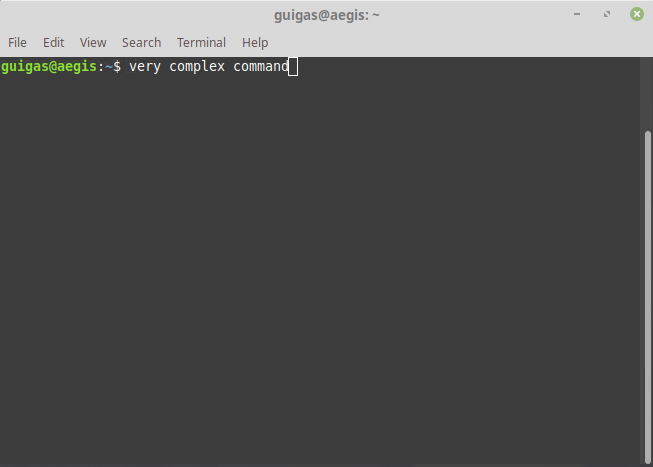
\includegraphics[width=\linewidth]{term2.png}
		\caption{A figura mostra a interface gráfica de um terminal atual.}
		\label{fig:term1}
	\end{figure}
	\subsection{Console}
	Então, terminal é um meio de acesso a um console, mas os comandos que você insere também não são do console, e sim do Shell, mas voltando ao console, não é necessário um terminal para acessar um console conforme a figura \ref*{fig:shellstruct}. Em um sistema linux, apertando "ctrl" + "alt" + "F1 , F2 , ... , F6" é possível acessar um dos consoles (F7 para sair). Hoje, isso também é conhecido como o modo texto do seu sistema operacional, pois é mais intuitivo que usar o termo console. Se um terminal era uma estação com tela e teclado, o console era a conexão física e digital entre o terminal e o mainframe. Então, Para cada sistema existe um console diferente, ligando cada sistema, a uma interface (geralmente, de texto), existem diferentes consoles que servem como interfaces para diferentes sistemas: BIOS, Boot Loader, init (processo incial do boot de sistemas unix). O console que está em uso quando você usa um terminal te da acesso ao Shell.
	\subsection{Shell}
	Shell possui esse nome pois ele funciona como uma casca separando o kernel do exterior. Sua função é servir de interface para acessar as funções do sistema operacional, tendo a vantagem de funcionar da mesma maneira em qualquer sistema operacional baseado em unix, escondendo detalhes específicos de cada SO.
	Portanto, os comandos que você insere no terminal, são comandos do Shell que você está utilizando, que, na maioria dos sistemas linux atualmente, é o Bash. Diferentes Shells possuem funcionalidades diferentes, possivelmente implementadas com comandos diferentes, essas funcionalidades incluem:
	\begin{itemize}
		\item Executar comandos.
		\item Manipulação de diretórios.
		\item Controle de processos (jobs).
		\item Expansões.
		\item Redirecionamento.
		\item pseudônimos (aliases).
		\item Histórico de comandos.
	\end{itemize}
	E muitas outras funcionalidades para facilitar, agilizar e automatizar as atividades realizadas.\\
	Essas são algumas funcionalidades que estamos acostumados a utilizar hoje, mas nas primeiras versões de Shell, muitas delas não existiam
	\\
	\begin{figure}[h]
		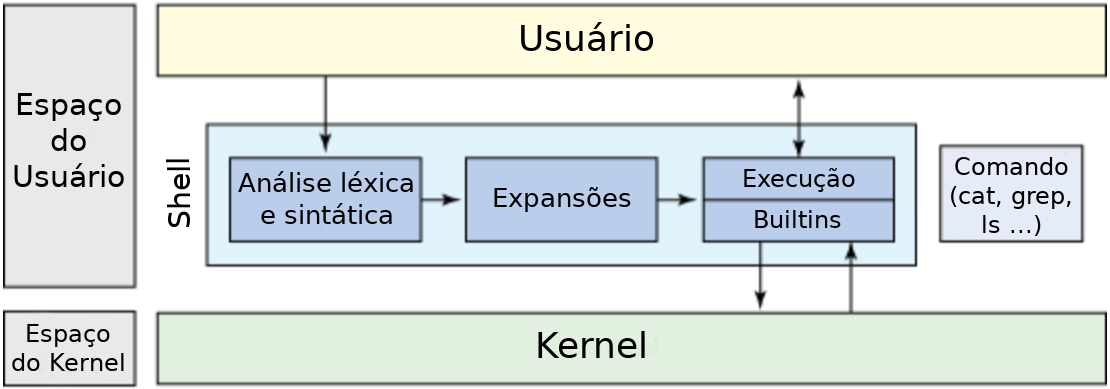
\includegraphics[width=\linewidth]{shell_struct1.png}
		\caption{Relação entre Shell, Kernel e usuário}
		\label{fig:shellstruct}
	\end{figure}
	
	\section{Unix, GNU, Linux e Shell}
	Em 1971, Ken Thompson desenvolveu o primeiro UNIX Shell, chamado de V6 Shell (foi criado no Unix versão 6), e suas funcionalidades muito básicas, ele permitia pipes e redirecionamentos, mas ele estava mais próximo de um interpretador de comandos, ao invés de scripts\par
	Dessa necessidade surgem novos Shells, com novas funcionalidades. Em 1977 foi criado o Bourne Shell, com dois objetivos: Servir como um interpretador de comandos e rodar scripts. Além disso, o Bourne Shell acrescentou ferramentas de controle (até então "if" existia como uma extensão, mas não era implementado diretamente no Shell V6), loops e variáveis, facilitando o uso de comandos e a criação de scripts. A partir disso surgem muitos outros Shells, e todos seguiram essas funcionalidades. Os principais foram: C-Shell, com o objetivo de deixar os scripts mais parecidos com a linguagem C. Korn Shell, que adicionou novas funcionalidades ao mesmo tempo que manteve forte compatibilidade com o Bourne Shell, e por fim, o Bourne Again Shell (Bash), que além de manter a compatibilidade com o Bourne Shell, também implementou as funcionalidades do C-Shell e Korn shell, ele também continuou a evoluir com o tempo, porém, um dos grandes facilitadores para o Bash ser o mais usado dos 3 é o fato de ele ser um projeto Open Source do GNU. \par
	O projeto GNU não se trata apenas de criar uma versão open source do UNIX, mas sim de criar um ambiente onde sistemas abertos respeitam especificações e padrões, de modo que os usuários tivessem a liberdade para escolher, usar, distribuir e modificar software, e para isso é necessário que todo o sofwate: Sistema operacional, drivers, programas fossem software livre. Para isso a criação do Bash foi necessária, e com o sucesso do \cite{gnu}, o Bash foi o Shell mais difundido.
	\section{Shell na atualidade}
	Ainda existem Shells sendo criados até hoje, geralmente adicionando funcionalidades para
	facilitar o uso das ferramentas já existentes no Bash, por exemplo, o Z shell (zsh) permite
	que usuário selecione o resultado das expansões de nomes de arquivos antes de executar o
	comando, além disso, quando o usuário digita parte de um caminho da árvore de diretórios,
	o zsh deixa visível os arquivos e diretórios visíveis à partir do caminho digitado, assim,
	unindo a intuitividade da interface gráfica com a agilidade da interface textual.
	
	A maior evolução de qualquer Unix Shell foi a ideia de transformar o shell em uma ferramenta para Scripts, e não apenas um interpretador de comandos, essa mudança surgiu no Bourne Shell, e é bem provável que, qualquer que seja o Shell mais comum no futuro, continue sendo algum derivado do Bourne Shell.
	
	\newpage
	\part{Uso Básico do Bash}
	
	Se você já precisou usar comandos do Bash para buscar partes específicas de um arquivo de texto, você sabe que muitas vezes é necessário usar mais de um comando, e simplesmente não é prático usar vários arquivos intermediários para chegar no seu resultado final.
	
	\section{Estrutura dos comandos do Bash}
	Uma linha de comando consiste de uma ou mais palavras, separadas por espaços. A primeira palavra é o próprio comando, seguido de um ou mais parâmetros(alguns comandos não exigem nenhum parâmetro). Um tipo comum de parâmetros são as opções, geralmente na forma de um traço seguido de uma letra. Algumas opções têm seus próprios parâmetros. Para exemplificar, vamos usar um comando que ordena linhas, o "sort". Suponha que queremos ordenar as linhas de um arquivo chamado lista.txt e queremos uma ordenação numérica, para isso usamos o seguinte comando:
	\begin{lstlisting}
	sort -n lista.txt
	\end{lstlisting}
	Neste caso, "sort" é o comando, "-n" é a opção que indica ordenação numérica e o "lista.txt" é o parâmetro que seleciona qual arquivo deve ser ordenado.
	Para saber quais opções e quantos parâmetros um comando pode ter, utilize o comando man, que também detalha o funcionamento do comando, então, em caso de dúvidas sobre como usar algum comando, leia a man page. basta digitar:
	\begin{lstlisting}
	man comando # troque "comando" pelo comando a ser  consultado
	\end{lstlisting}
	Neste caso, "man" é o comando e "comando" é o parâmetro para escolher qual man page deve ser consultada. Além disso, o conteúdo da linha à partir do '\#' é lido como comentário.
	
	\section{Arquivos e Diretórios}
	 A seção anterior explica como usar qualquer comando, porém, o Bash não se tornou o Shell mais utilizado por ser um simples interpretador de comandos.Em sistema UNIX, o conceito de arquivo é bem amplo, não há nenhuma estrutura definida, o significado da sequência de bytes armazenada em um arquivo, é dependente de qual aplicação o utiliza. O nome do arquivo também não é definido. Todo tipo de padrão como headers, conteúdo e extensões(".txt, .mp3") são maneiras de organizar os arquivos. É possível separar os tipos de arquivos em 3:
	\begin{itemize}
		\item Arquivo de texto, que contém caracteres legíveis.
		\item Arquivo executável, o conteúdo desse tipo de arquivo não são caracteres legíveis, então não é uma boa ideia abrir um arquivo como esse em um editor de texto.
		\item Diretório. Conhecidos pela abstração "pasta". São criados para guardar outros arquivos (qualquer tipo, até outros diretórios).
	\end{itemize}
	\subsection{Navegação}
	Uma abstração importante dos sitemas UNIX é a árvore de diretórios. Mesmo que os dados não sejam armazenados dessa forma, diretórios possuem uma estrutura hierárquica, onde um diretório é o pai de todos os diretórios que ele contém. Diretórios são irmãos, se possuem o mesmo pai, além disso, diretórios possuem apenas um pai. O diretório raiz é chamado "root".
	
	Para poder navegar pela árvore de diretórios e não precisar saber ou digitar o caminho completo de um arquivo, existe o conceito de diretório atual, assim, é possível se referir a arquivos tanto de maneira relativa a esse diretório quanto de maneira absoluta(partindo do root, para isso, o caminho deve começar com uma barra (/)). Os caminhos são compostos de diretórios separados por barra. Para que um caminho seja válido, os diretórios em sequência, devem possuir uma conexão na árvore de diretórios.
	
	Além disso, Todo diretório possui uma conexão ao diretório pai (..) e a si mesmo (.), assim, é possível acessar qualquer diretório, a partir de qualquer outro diretório, porém, caso o diretório corrente seja um diretório profundo de um ramo da árvore, pode ser mais rápido acessar o diretório desejado pelo seu caminho absoluto, partindo da raiz, ao invés de retornar vários diretórios usando "..".
	
	Além da árvore de diretórios e do diretório atual, no UNIX, cada usuário possui um diretório "home", esse diretório serve para separar os arquivos do sistema, executáveis de programas, e outros arquivos, dos diretórios pessoais do usuário. Convenientemente, um usuário logado possui um atalho para a sua home, sendo assim, ele sempre pode se referenciar a sua home com o caractere TIL (\texttildelow).
	Exemplos: 
	\begin{lstlisting}
	/home/usuario/Documentos
	../../media/dispositivo
	~/Downloads
	\end{lstlisting}
	Os comandos da tabela \ref{table:1} são os mais usados para navegação na árvore de diretórios:
	
	\begin{table}[!ht]
		\centering
		\begin{tabular}{ | c | c | } 
			\hline
			\bfseries Nome do comando & \bfseries Função \\
			\hline
			pwd & Retorna o diretório atual \\
			\hline
			ls & Lista os arquivos de um diretório \\
			\hline
			cd & Muda o diretório atual \\
			\hline
			mkdir & Cria um novo diretório \\
			\hline
		\end{tabular}
		\caption{Comandos de navegação}
		\label{table:1}
	\end{table}
	O comando ls pode ser usado no diretório atual ao omitir o parâmetro de localização, existem opcionais para mostrar metadados e incluir arquivos ocultos (arquivo cujo nome começa com ponto (.)). O comando cd aceita tanto caminho absoluto quando caminho relativo. Ao omitir o parâmetro de localização o diretório atual será a home. Mais detalhes sobre as opções e parâmetros dos comandos podem ser encontrados nas man pages. O mesmo vale para os comandos apresentados até o fim desse material. É indicado que o leitor teste o que é apresentado nesse material, lendo as man pages e testando opções dos comandos.
	
	Dica: Utilize o auto-complete para evitar digitação desnecessária! TAB para completar quando há apenas uma opção possível e TAB duas vezes para mostras as opções possíveis, tanto para completar comandos quanto para nomes de arquivos e diretórios existentes e acessíveis no caminho digitado(na verdade, os comandos também são arquivos, os comandos do Bash ficam no diretório /bin).
	\section{Expansão}
	A seção anterior detalha como navegar na árvore de diretórios, porém, muitas vezes não mantemos um mapa mental completo da árvore e nesse caso a navegação, mesmo com auto-complete ainda é muito precária. Esse é um dos usos dos caracteres coringas, ou, "meta-caracteres".
	
	O asterísco (*) substitui qualquer sequência de caracteres e o ponto de interrogação (?) substitui um único caractere. Então, suponha que em seu diretório atual, existem os seguintes arquivos: b16c8a16.txt, b4c4a32.txt e b128c2a8.txt, suponha também uma infinidade de arquivos com nomes variados de modo que ls não é a forma mais rápida de identificar arquivos. com o asterísco, é possível selecionar um arquivo sabendo apenas parte de seu nome, por exemplo, o comando "ls b16*" retornaria apenas o arquivo b16c4a32.txt (caso nenhum outro arquivo do diretório corrente comece com b16). o comando "ls b1?c" retorna apenas o arquivo b16c8a16.txt. Usando um "*" no lugar do "?", o comando retornaria tanto o arquivo "b16c8a16.txt" quanto o "b128c2a8.txt".
	
	Suponha agora que você quer imprimir o conteúdo de todos os arquivos que acabam em ".txt". O comando cat imprime o conteúdo de um arquivo na tela. Caso o usuário não saiba o nome de todos os arquivos(ou apenas não queira digitar todos), mesmo que sejam muitos arquivos, ainda é possível realizar essa tarefa apenas com o seguinte comando:
	\begin{lstlisting}
	cat *.txt
	\end{lstlisting}
	Com os comandos mv(mover) e cp(copiar) é possível realizar rapidamente tarefas bem comuns de gestão de arquivos. É indicado que o leitor crie um diretório para testar comandos com '*' e '?', em especial com o comando rm (remover). Cuidado com o uso de ".*", lembre dos diretórios . e .. antes de executar comandos destrutivos.
	
	Com o uso dos colchetes ('[' e ']') é possível criar coringas mais específicos para a expansão de caminhos, por exemplo, a expansão *.[abc] funciona para todos os 3 casos: "*.a", "*.b" e "*.c". A tabela \ref{table:2} possui mais exemplos de expansão, lembre que a expansão de colchetes corresponde a um único carectere:
	\begin{table}[!ht]
		\centering
		\begin{tabular}{ | c | c | } 
			\hline
			\bfseries Expansão & \bfseries corresponde à \\
			\hline
			[b-e.;!] & Qualquer letra minúscula de "b" a "e", ".", ";" e "!" \\
			\hline
			[!b-e] & Qualquer dígito, exceto letras minúsculas de "b" a "e" \\
			\hline
			[A-Z0-9] & Qualquer letra maiúscula de "A" a "Z" e qualquer número de um dígito \\
			\hline
			[a-df-i] & a, b, c, d, f, g, h, i \\
			\hline
			[abc-] & 'a', 'b', 'c', ou '-' \\
			\hline
		\end{tabular}
		\caption{Expansão de caminhos}
		\label{table:2}
	\end{table}
	
	
	Expansão de caminhos é o primeiro passo para fazer scripts em Bash, com eles é possível realizar ações para várias entradas, de uma só vez. Porém, nem todo parâmetro é um nome de arquivo ou diretório, para isso existe a expansão de chaves ('\{' e '\}'), que permite a expansão para um conjunto de strings, separadas por ','. Apesar de funcionar de maneira parecida, nesse tipo de expansão, não há a necessidade de corresponder com nomes de arquivos existentes. A tabela \ref{table:3} contém exemplos de uso da expansão de chaves:
	
	\begin{table}[!ht]
		\centering
		\begin{tabular}{ | c | c | } 
			\hline
			\bfseries Expansão & \bfseries Resultado \\
			\hline
			cat func.\{c,h\} & conteúdo dos arquivos fun.c func.h \\
			\hline
			ls rec0\{1..4\}.mp3 & rec01.mp3 rec02.mp3 rec03.mp3 rec04.mp3 \\
			\hline
			\multirow{2}{13em}{touch 201\{5..7\}/ex\{1..4\}.txt} & cria ex1.txt, ex2.txt, ex3.txt e ex4.txt \\ 
			& nos diretórios 2015, 2016 e 2017 \\
			\hline
			echo turma\{A..D\} & turmaA turmaB turmaC turma D\\
			\hline
			echo turma\{A..G..2\} & turmaA turmaC turmaE turma G\\
			\hline
		\end{tabular}
		\caption{Expansão de chaves}
		\label{table:3}
	\end{table}
	Se necessário, consulte as man pages dos comandos echo e touch. Com a expansão de chaves é possível expandir caminhos que não existem, então dependendo do caso você pode obter respostas de erro do comando utilizado.
	
	As mensagens de erro dos comandos do Bash são bem intuitivas, antes de ir ao google, leia a mensagem de erro, e se necessário a man page. Para os casos comuns, isso basta.
	
	Em caso de dúvidas nos resultados das expansões, use o comando echo para conferir se a expansão gera o resultado esperado, antes de usar a expansão em comandos que podem estragar ou mover arquivos importantes. Lembre-se da diferença entre a expansão de chaves da expanção de colchetes.
	\section{Redirecionamento de Entrada e Saída}
	Os redirecionamentos são o próximo passo da evolução de comandos para scripts. As expansões são muito úteis, mas nem tudo pode ser resolvido com apenas um comando. Uma ótima abstração para entender a funcionalidade do redirecionamento no Bash é pensar nos comandos como filtros. Um comando recebe uma entrada e produz uma saída, até esse ponto do material a entrada era sempre lida pelo teclado (stdin - Standard Input) e imprimidas na tela (stdout - Standard Output), porém, se é possível usar comandos como filtros, podemos redirecionar a saída de um comando para a entrada de outro, e assim, combinar vários comandos para obter a saída desejada, com uma estrutura parecida com essa:
	
	\begin{lstlisting}
	entrada -> Filtro1 -> Filtro2 -> ... -> FiltroN -> saída
	\end{lstlisting}
	A notação para redirecionamento de entrada é '<' e, '>' para saída. Então, o seguinte exemplo redireciona a saída do comando cat para o arquivo teste.txt:
	
	\begin{lstlisting}
	cat texto.txt > teste.txt
	\end{lstlisting}
	Também é possível redirecionar a entrada de um comando. Suponha um programa que lê na entrada padrão. Caso hajam muitas entradas de teste ou caso a entrada seja muito grande. É possível redirecionar um arquivo como entrada dessa forma:
	
	\begin{lstlisting}
	./programa < entrada1.txt
	\end{lstlisting}
	Observação: './' é a maneira de executar um arquivo executável (tente './ls' no diretório '/bin').
	
	A última ferramente para usar programas e comandos como filtros, como exemplificado anteriormente é o pipeline (|). O pipeline elimina a necessidade de arquivos intermediários e liga diretamente a saída de um programa a entrada de outro conforme o exemplo:
	
	\begin{lstlisting}
	ls /dev | grep std | tee file1.txt file2.txt file3.txt
	\end{lstlisting}
	O resultado desse comando imprime 3 arquivos: 'stdin', 'stdout' e 'stderr'. O terceiro ainda não foi apresentado nesse material. stderr é, por convenção, o local para imprimir warnings e erros dos programas, como um log.
	O comando grep seleciona apenas as linhas do resultado que contém a substring passada como parâmetro. O comando tee redireciona a entrada para todos os arquivos passados como parâmetro.
	
	Um uso comum do pipeline é filtrar diferentes dados dos nomes de arquivos partindo do comando ls, ou do conteúdo desses, partindo do comando cat, e utilizar os comandos grep, cut e tr, respectivamente para filtrar linhas específicas, filtrar seções de uma linhas e substituir caracteres, e, ao final é possível redirecionar a saída para um arquivo.
	
	\section{exercício}
	
	\begin{enumerate}
		\item Utilizando apenas um comando mkdir e expansão de chaves, crie os 7 diretórios com os seguintes nomes: 3 diretórios para turmaAP, turmaREP e turmaFN e os 3 diretórios turmaA, turmaB e turmaC 1 diretório de nome alunos. Dentro de um diretório seguro para testes.
		
		Resposta:
		\begin{lstlisting}
		mkdir turma{{A..C},{AP,REP,FN}} alunos
		\end{lstlisting}
		\item dentro do diretório alunos, crie arquivos de nome de alunos no formato aluCnotaN para cada curso C entre: BCC, IBM, TADS e OUTRO e para cada nota N entre 0 a 10 e NULL. Exemplo de arquivo: aluBCCnotaNULL
		
		Resposta:
		\begin{lstlisting}
		touch alunos/alu{BCC,IBM,TADS,OUTRO}nota{{0..10},NULL}
		\end{lstlisting}
		\item Copie os arquivos do diretório alunos para o diretório correspondente de acordo com a tabela \ref{table:4}:
		
		\begin{table}[!ht]
			\centering
			\begin{tabular}{ | c | c | c | } 
				\hline
				\bfseries Exercício & \bfseries Arquivos & \bfseries Copiar para \\
				\hline
				3.1 & Alunos de BCC com nota diferente de NULL & turmaA \\
				\hline
				3.2 & Alunos de IBM com nota diferente de NULL & turmaB \\
				\hline
				3.3 & Alunos de TADS com nota diferente de NULL & turmaC \\
				\hline
				3.4 & Alunos de BCC, IBM e TADS com nota de 0 a 3 & turmaREP \\
				\hline
				3.5 & Alunos de BCC, IBM e TADS com nota de 4 a 6 & turmaFN \\
				\hline
				3.6 & Alunos de BCC, IBM e TADS com nota de 7 a 10 & turmaAP \\
				\hline
			\end{tabular}
			\caption{Relação de arquivos e destinos}
			\label{table:4}
		\end{table}
		Resposta:
		\begin{lstlisting}
		cp alunos/aluBCCnota[!A-Z]* turmaA/
		cp alunos/aluIBMnota[!A-Z]* turmaB/
		cp alunos/aluTADSnota[!A-Z]* turmaC/
		cp alunos/alu{BCC,IBM,TADS}nota[0-3] turmaREP/
		cp alunos/alu{BCC,IBM,TADS}nota[4-6] turmaFN/
		cp alunos/alu{BCC,IBM,TADS}nota{7..10} turmaAP/
		\end{lstlisting}
	\end{enumerate}
	
	As ferramentas do Bash apresentadas nesse material, juntamente com estruturas de controle
	(if e for) e variáveis, permitem que sejam criados scripts que interagem dinamicamente com
	os dados sem excesso de digitação e trabalho por parte do usuário. Para que esse conteúdo
	seja entendido pelo leitor é ideal que os conhecimentos sejam aplicados na prática. Para isso,
	são indicados os materiais do professor Roberto Hexsel \cite{roberto1, roberto2}, além
	de serem bem explicativos, possui vários exemplos, explicam novos comandos e possuem
	alguns exercícios para praticar.
	
	\newpage
	\part{Customização do ambiente}
	
	A seção seguinte explica os métodos de customização do Shell, sem a intenção de listar e detalhar as opções, porém, bibliografias para consulta das opções serão indicadas. Alguns desses métodos são utilizados por outras aplicações como editores de texto.
	
	\section{Introdução}
	As duas principais maneiras de customização do bash são opções e variáveis de ambiente, algumas opções são definidas com o comando set, outras com o comando shopt (shell options), e as variáveis de ambiente são variáveis definidas sempre que o bash inicia a execução. Opções e variáveis podem ser alteradas pelo usuário a qualquer momento, mas, para que não seja necessário configurar o bash toda vez ao abrir um bash, elas podem ser definidas nos arquivos: .bash\_profile e .bashrc. Para explicar o funcionamento desses arquivos, antes é necessário definir as variáveis do Bash.
	
	\section{Variáveis e Aliases}
	Para auxiliar os scripts no Bash, variáveis servem para guardar qualquer tipo de valor, incluíndo retorno de programas\footnote[1]{Para atribuir o retorno da execução de um programa em uma variável, deve-se englobar a execução no seguinte formato: variavel=\$(execução)}. A sintaxe para definir variáveis é: \texttt{\textbf{\textit{nome=valor}}}, sem espaços antes ou após o '=', e se o valor contém um ou mais espaços, o valor deve estar entre aspas\footnote[2]{Aspas simples para o valor literal da string e aspas duplas para realizar expansões e traduzir valores de variáveis dentro do conteúdo}. Para obter o valor de uma variável, a sintaxe é \texttt{\textbf{\textit{\$nome}}}.
	
	De maneira similar é possível definir aliases, para encurtar comandos muito usados que são difíceis de digitar. Por exemplo, é possível definir que o comando \texttt{\textbf{\textit{pr * | lpr}}} será executado ao digitar \texttt{\textbf{\textit{pa}}}, usando o comando: \texttt{\textbf{\textit{alias pa='pr * | lpr'}}}. É importante ressaltar que aliases podem ser usados apenas no início de um comando, e apesar de existirem outras formas de contornar os problemas gerados por essa limitação, nas próximas partes desse material, serão apresentadas as funções, que permitem mais flexibilidade que os aliases.
	
	\section{Os arquivos de configuração e Run-Control}
	Existem dois arquivos para customizar o shell, o primeiro deles é o profile, situado no diretório home de cada usuário, geralmente usado para definir variáveis de ambiente e opções, como definições padrão e escolhas de método de funcionamento do bash. Uma lista de variáveis pode ser encontrada, digitando:
	\begin{lstlisting}
	compgen -v | while read line; do echo \$line=\${!line};done
	\end{lstlisting}
	O comando while está sendo utilizado apenas para imprimir conteúdos de variáveis que contém mais de uma linha. Mais detalhes sobre o comando while serão tratados nas próximas partes desse material.
	A lista de opções pode ser encontrada no manual de referencia do bash\cite{bashman}, nas seções 4.3.1 e 4.3.2.
	Existem muitas opções e variáveis de ambiente, por isso, é mais produtivo que o autor procure por elas de acordo com a necessidade de alguma configuração específica. Esse não é o caso para a variável \$PATH, pois algumas aplicações exigem que o usuário altere seu conteúdo, essa variável contém os caminhos dos arquivos executáveis, então se você quer tornar executáveis próprios acessíveis sem a necessidade de referenciar o caminho até o executável, é indicado criar um diretório para esses executáveis, e adicionar o caminho desse diretório à variável \$PATH. Para adicionar um caminho à variável PATH sem sobrescrever seu conteúdo, atribua \texttt{\textbf{\textit{PATH=\$PATH":/home/caminho/do/diretorio"}}}.
	
	Outro arquivo de customização do bash é o .bashrc, também situado na home do usuário. Esse arquivo geralmente contém definições de preferências pessoais, como mudar o prompt, ou mudar as cores além da definição de aliases. O .bashrc é um arquivo de run-control, usados por diversas aplicações como um arquivo de declarações e comandos, associados ao programa que o interpreta na inicialização\footnote[3]{Geralmente sistemas possuem um arquivo de run control com definições compartilhadas para todos os usuários, e outro, na home de cada usuário, para definições pessoais}. O processo de inicialização, que inclui como o bash interpreta as definições desses dois arquivos é detalhada na seção seguinte.
	
	O conteúdo dos dois arquivos de configuração é apenas uma convenção de boa prática para facilitar a identificação dessas configurações. Idealmente as alterações devem ser seguidas de comentários. Como dito antes, esse material não descreve cada opção de configuração, isso porque são tantas opções que dificilmente o leitor não lembraria de cada detalhe quando seu uso fosse necessário, o mesmo acontece para para os arquivos de configuração, caso seja necessário retornar à configuração, um comentário relembrando a necessidade de cada linha é muito bem vindo.
	
	Ainda existe o arquivo .bash\_logout para as definições e principalmente execução de scripts que é executado ao encerrar a execução do Bash.

	\section{Inicialização do Bash}
	Para reforçar, um shell interativo é aberto ao shell através de um terminal, e quando o acesso ao shell exige um login e senha, como no acesso através do modo texto ou ssh, esse é chamado de login shell.
	
	Ao iniciar um login shell, após a autenticação, o shell executa o script /etc/profile, que inicializa variáveis necessárias e executa os scripts (*.sh) do diretório profile.d. Qualquer alteração nesse procedimento deve ser incluída como um script nesse diretório, para que alterações no /etc/profile não sejam sobrescritas em alguma atualização do sistema. Por fim, o perfil pessoal do usuário, que, devido à retro-compatibilidade do bash, pode possuir diferentes nomes, será executado. A ordem de prioridade entre os arquivos de perfil de usuário, da maior para a menor, é:
	
	\begin{samepage}
		\begin{itemize}
			\item .bash\_profile
			\item .bash\_login
			\item .profile
		\end{itemize}
	\end{samepage}
	Sendo que apenas o arquivo encontrado de maior prioridade será executado.
	
	Ao final da execução do perfil do usuário, o arquivo .bashrc é executado (lembre-se de manter essa definição, ao editar seu profile), também contendo definições específicas do usuário. Em alguns sistemas, também é executado o bashrc compartilhado a todos os usuários.
	
	Para a inicialização de um Shell interativo o processo é mais simples: Os arquivos bashrc são executados (o arquivo para todos os usuários e o específico do usuário que abriu o bash), mesmo que essa execução não seja especificada no .profile, pois a execução do bashrc é realizada diretamente pelo shell interativo.
	
	Como esperado, o bash não possui um menu gráfico com botões e opções de configuração, ao invés disso, o usuário pode configurar o bash através de variáveis pré-definidas e opções (set e shopt). Para que não seja necessário configurar o bash toda vez que o bash é inicializado, existem os arquivos de perfil e o run control .bashrc. Pela maneira que esses arquivos são executados, suas alterações não serão refletidas em shells iniciados antes da alteração.
	
	O uso de arquivos run control não é exclusivo do bash e se encontra até em editores de texto como o Vim, a lista de opções de configuração do vim podem ser encontradas no manual de referência do vim \cite{viman}. O escopo desse material é apenas de informar os meios de configuração e o funcionamento do sistema de configuração. É ideal que o leitor se acostume com o fluxo de encontrar uma necessidade e buscar uma configuração para atender essa necessidade.
	
	\newpage
	\part{Shell e Linux sem Mouse}
	
	Esta seção mostra alguns atalhos específicos de aplicações, especialmente do linux mint, porém, muitas ações realizadas por atalhos funcionam da mesma forma com outro atalho em aplicações similares, mesmo em outras distribuições do linux ou em outros sistemas operacionais.

	O uso do shell para realizar atividades repetitivas (ou com algum padrão definido) se provou ser bem mais eficiente que o sistema de apontar e clicar, usado como método principal de entrada de comandos na maioria das interfaces mais usadas atualmente. Apesar do mouse ser muito simples e intuitivo de usar, é comum que usuários mais experientes busquem modos mais rápidos de realizar as mesmas ações. Felizmente, é possível identificar padrões nos principais atalhos do teclado em diferentes interfaces, muitas interfaces, usam o mesmo atalho para ações similares, independente do sistema, e algumas vezes é possível inferir um comando pela inicial da ação a ser realizada.
	
	\section{Atalhos do Sistema}
	Esse material se limita a focar no Linux Mint, mais especificamente com o ambiente Cinnamon, pois é uma distribuição extremamente fácil de usar para usuário iniciantes e é a distribuição mais acessível para calouros do curso de Ciência da Computação na UFPR. Os atalhos mais importantes do sistema para usuário do shell são atalhos de manipulação de janelas, pois a maneira mais eficiente de usar o shell, geralmente é usando mais de um shell ao mesmo tempo. Os atalhos da tabela \ref{table:5} são os principais atalhos do Linux Mint, com ambiente desktop Cinnamon:
	
	\pagebreak
	
	\begin{table}
		\centering
		\begin{tabular}{|c|p{10.0cm}|}
			\hline
			\bfseries Combinação de teclas & \bfseries Função \\ \hline
			super seta & Expande ou encolhe a janela atual para a direção inserida \\ \hline
			super d & Alterna entre a área de trabalho e as janelas abertas \\ \hline
			alt F4 & Fecha a janela atual \\ \hline
			alt tab & Alterna entre as janelas abertar, começando da janela atual até a janela menos recente\\ \hline
			alt shift & Alterna entre as janelas abertar, na ordem inversa\\ \hline
			ctrl alt backspace & Fazer log off no sistema \\ \hline
			ctrl d & Equivalente ao comando exit, no shell. \\ \hline
			ctrl alt t & Abre um terminal \\ \hline
		\end{tabular}
		\caption{A tabela mostra a combinação das teclas, suas respectivas funções e interfaces onde podem ser utilizados}
		\label{table:5}
	\end{table}
	
	É importante notar que a criação de atalhos de teclado padrão geralmente é originada usando a inicial da palavra (em inglês) que descreve a função do atalho, por exemplo, em editores de texto, as funções de Negrito, Itálico e Sublinhado, se originam das palavras bold, italic e underline, e portanto seus atalhos são, respectivamente ctrl b, ctrl i e ctrl u. Em alguns editores, quando usados em português, existem dois atalhos para negrito, ctrl b e ctrl n, para servir tanto aos usuários que já usam editores que possuem esse padrão, quanto para usuário que tentam inferir o atalho pelo nome da funcionalidade em português.
	
	Nem sempre é possível inferir o atalho pelo nome, isso porque sua origem é legado de programas antigos que criaram o padrão que é usado atualmente, ou porque já existe uma funcionalidade mais básica que ocupa esse atalho. Nesse caso é possível buscar atalhos com funções similares de outras aplicações e interfaces ou ler o menu de ajuda / manual, ou mesmo pesquisando na internet.
	
	\section{Uso do Sistema}
	Um fluxo de trabalho comum é abrir uma aplicação e carregar um arquivo através dos menus dessa aplicação. O Linux Mint possui uma maneira rápido de realizar a primeira tarefa sem o uso do mouse. Apertando o botão super, o menu de aplicações se sobrepõe à tela e permite ao usuário digitar o nomes de aplicações, menus do sistema e os principais diretórios da home do usuário. Dessa maneira, é possível abrir aplicações apenas com o teclado. Além disso, é possível navegar pela maioria dos menus do sistema usando as setas, "tab" / "ctrl tab" ("shift tab" / "ctrl shift tab" para mover na ordem reversa) e outros atalhos utilizados na maioria das interfaces gráficas. Por exemplo, a interface gráfica do navegador de arquivos do sistema pode ser utilizado completamente pelo teclado. Usando as setas para selecionar arquivos, "enter" para abrir arquivos ou avançar para um diretório, "backspace" para retornar ao diretório pai, "ctrl a" para selecionar todos os arquivos e diretórios, segurar "shift" para realizar uma seleção de multiplos arquivos em sequência e "ctrl w" para fechar. Dessa forma, mesmo quando interfaces exigem que o usuário busque um arquivo através do navegador de arquivos, o mouse não é necessário. Outras interfaces gráficas possuem sistemas de navegação parecido, e muitas vezes, as opções do menu possuem um atalho atribuido, de modo que os usuários que usam o mouse possam se acostumar com os atalhos das opções que utilizam.
	\begin{figure}[h]
		\centering
		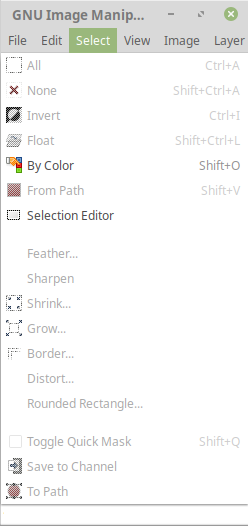
\includegraphics[width=4.0cm]{shotc.png}
		\caption{A figura mostra um exemplo de atalhos referentes às opções de menu.}
		\label{fig:shortc}
	\end{figure}
	
	Outro fluxo de uso comum é buscar um arquivo pelo navegador de diretórios do sistema e abrir o arquivo desejado diretamente com a aplicação escolhida. Isso pode ser feito de maneira mais rápida com o shell, aplicações comuns podem ser iniciadas pelo shell com seus comandos, por exemplo, o comando vlc Downloads/Music abre o programa vlc, com as músicas do diretório (e dos diretórios filhos de) Downloads/Music. Adicionando o caracter '\&', o comando executa no background, sendo possível continuar usando o mesmo shell. Se necessário, é possível redirecionar a saída desse comando para /dev/null para ignorar algumas mensagens que o comando pode retornar durante a execução.
	Para encontrar arquivos, é possível usar o comando find, passando o diretório de partida e uma expressão regular, ou mesmo utilizar das expansões do bash.
	Caso o usuário não conheça o comando para abrir o arquivo desejado, é possível usar o comando gnome-open para abrir o arquivo com uma aplicação inferida através da extensão ou cabeçalhos do arquivo. Devido à existência de outros comandos começados em "gnome-" é recomendada a criação de um alias para esse comando.
	
	\section{Terminal}
	O Shell possui muitas maneiras de facilitar e agilizar tarefas e o sistema possui seus próprios atalhos de navegação entre janelas, mas ainda existem atalhos implementados pelo terminal, a interface gráfica do shell. Como é comum utilizar mais de um shell simultaneamente, o próprio terminal possui a funcionalidade de abrir abas, com o atalho "ctrl shift t". Para alternar entre as abas existentes é possível usar os atalhos "ctrl page up" e "ctrl page down" para, respectivamente, mudar para a próxima aba, ou para a aba anterior. Também é possível navegar pelas abas usando com "alt num", trocando "num" pelo número da aba desejada.	
	
	É ideal que o usuário busque conhecer os atalhos disponíveis sempre que realizar alguma ação demorada que poderia ser encurtada. A maioria das aplicações possuem atalhos em comum e muitas ainda permitem a criação ou alteração de atalhos. Diferente do mouse, o uso do sistema apenas com o teclado não é tão intuitivo, porém, com um pouco de aprendizado e prática, ele é muito mais rápido e exige menos esforço. A maior fonte de perda de tempo dos usuários iniciantes é edição de código fonte, as formas de agilizar a edição vão muito além do autocomplete oferecido pela maioria dos editores de texto de interface gráfica.
	
	\section{Editor de texto}
	O vim é um editor de texto para usuários de shell, em outras palavras, um editor que não possui uma interface gráfica e menus, porém, com atalhos, comandos e opções que permitem ao usuário configurar o ambiente e preferências além da edição de texto de forma eficiente. Assim como o bash, o vim não é intuitivo para usuários iniciantes, para isso, é recomendado um tutorial interativo \cite{vimt}. Além disso, o vim é configurável com um arquivo run command vimrc, e os comandos de configuração também podem ser inseridos durante a execução.
	
	\pagebreak
	\part{Controle de Processos}
	
	Ao executar algum comando\footnote{Vários comandos com pipelines e redirecionamentos são agrupados no mesmo processo} no bash, um processo é iniciado em primeiro plano (\textit{foreground}), interrompendo a execução do bash e podendo ler a entrada do teclado. É possível iniciar um processo (\textit{job}) no background pelo bash, inserindo o caractere '\&' ao final da linha de comando. Quando o bash cria um \textit{job} em segundo plano, ele imprime uma linha contando o número de sequência do \textit{job} e o process id do último processo do pipeline.
	
	\section{Comandos de Controle de Processos}
	Para facilitar o gerenciamento dos processos, o bash mantém o registro de um \textit{job} atual(último job interrompido em foreground ou último processo iniciado em background) e um \textbf{job} anterior.
	
	 Com o comando 'ctrl' 'z' na maioria dos terminais, o processo em primeiro plano é interrompido, liberando a leitura do teclado de volta ao bash. O comando 'fg' serve para executar um job em primeiro plano e o comando 'bg' para executar um job em segundo plano. O comando 'jobs' lista os jobs ativos. Ao finalizar um job em segundo plano, o bash imprime uma linha contendo o número de sequência do job e o comando com o qual ele foi invocado (para não interromper alguma execução em primeiro plano, essa impressão aguarda até que outra impressão seja realizada pelo bash).
	 
	 Os comandos 'fg' e 'bg' pressupõe o job atual quando não é passado nenhum parâmetro, mas é possível utilizar esses comandos em outros jobs com um jobspec. Um jobspec é uma referência a um job, ele começa com o caractere '\%' seguido do número de sequência do job, ou seguido do comando de invocação do job e é possível utilizar o caractere ? para utilizar uma substring do comando de invocação do job. \%+ é usado para se referir ao job atual e \%- para o job anterior.
	 Exemplos:
	 \begin{lstlisting}
	 	fg %5
	 	bg %vim
	 	fg %?vi
	 	fg %-
	 \end{lstlisting}
	
	Também é possível enviar um sinal a um job com o comando kill. Uma lista completa de sinais pode ser obtida com o comando \texttt{\textbf{\textit{kill -l}}}. O sinal mais comum é o SIGKILL (9), que força o encerramento da execução. 
	 
	O manual do bash \cite{bashman} explica em detalhes o funcionameto do controle de processos do bash na seção 7.1 e na seção 7.2 detalha o funcionamento de comandos de controle de processos. A seção 12 do manual Shell Scripting \cite{learnl} apresenta o funcionamento de vários sinais utilizados no comandos kill com exemplos de uso e exercícios, além de mostrar como tratar de forma diferenciada os sinais recebidos em um script(traps). O comando kill recebe o tipo de sinal enviado como opção e o um jobspec ou process id como parâmetro.
	
	Para poder enviar sinais a 
	
	
	\newpage
	\part{Exercício Prático 1}
	
	O exercício a seguir propõe ao leitor encontrar uma solução automatizada para filtrar e separar dados específicos de um arquivo, usando apenas o bash (e auxiliares, invocados pelo bash). A solução inclui a pesquisa por ferramentas que possam ser de auxílio na solução, como sed, awk, cut, entre outros (para usar o bash da melhor forma é preciso conhecer, ou ser capaz de pesquisar por, ferramentas que auxiliam as soluções).

	As expansões do Bash, juntamente com os redirecionamentos, são muito práticos, porém, para qualquer programador, é difícil automatizar tarefa sem utilizar estruturas de controle como 'if' e 'for' (while), por isso é difícil encontrar exemplos reais de uso para automatização que usem apenas as ferramentas apresentadas até o momento. Para o exercício seguinte não é necessário o uso de 'if', mas é recomendado o uso do 'for' para obter uma solução ideal. O material do prodessor Roberto Hexsel \cite{roberto3} apresenta com exemplos práticos e exercícios sobre o conteúdo necessário para a solução do exercício deste capítulo, incluíndo comando for e variáveis.
	
	\section{Exercício}
	Para um arquivo patrimonio.csv no seguinte formato:
	\begin{lstlisting}
	...
	"447676";"ARMARIO";"ALTO COM DUAS PORTAS";"";"2100.13.03.31";
	"447677";"ARMARIO";"ALTO COM DUAS PORTAS";"";"2100.13.03.29";
	"447678";"ARMARIO";"ALTO COM DUAS PORTAS";"";"2100.13.03.30";
	"447679";"ARMARIO";"ALTO COM DUAS PORTAS";"";"2100.13.03.28";
	"452782";"CADEIRA GIRATORIA";"BASE A GAS";"FUNPAR";"2100.13.07";
	"460805";"FORNO DE MICROONDAS";"30L";"CONSUL";"2100.13.02.24";
	"460806";"VENTILADOR DE TETO (5234)";"127V ";"";"2100.13.02.21";
	"460807";"VENTILADOR DE TETO (5234)";"127V ";"";"2100.13.02.21";
	"460808";"VENTILADOR DE TETO (5234)";"127V ";"";"2100.13.02.21";
	...
	\end{lstlisting}
	
	Em cada linha, o conteúdo das colunas está entre aspas ('' ''), separados por ponto e vírgula (;). Porém, o conteúdo de alguns campos pode conter o caractere (;). Exemplo:
	Original:
	\begin{lstlisting}
	"460808";"VENTILADOR DE TETO; CINZA";"127V ";"";"2100.13.02.21";
	\end{lstlisting}
	Filtrado:
	\begin{lstlisting}
	"460808";"VENTILADOR DE TETO CINZA";"127V ";"";"2100.13.02.21";
	\end{lstlisting}
	A primeira etapa do exercício é filtrar todo o conteúdo do arquivo e remover essas ocorrências. A segunda etapa, é, a partir do resultado filtrado, obter em um arquivo, todos os locais (conteúdo da quinta coluna), um em cada linha, ordenados e sem repetição.
	Exemplo:
	\begin{lstlisting}
	...
	2100.13.02.21
	2100.13.02.23
	2100.13.02.24
	2100.13.02.25
	2100.13.02.29
	2100.13.03.01
	2100.13.03.02
	2100.13.03.03
	2100.13.03.04
	...
	\end{lstlisting}
	Por fim, deve-se criar um arquivo para cada local, com o nome sendo o código do local com a extensão ''.csv''. O conteúdo de cada arquivo deve ser as linhas do arquivo original em que o campo de local corresponde ao nome do arquivo. Exemplo:
	2100.13.csv:
	\begin{lstlisting}
	...
	"480170";"NO-BREAK (5230)";"";"";"2100.13";
	"480171";"MICROCOMPUTADOR ";"";"";"2100.13";
	"480172";"NOTEBOOK";"";"";"2100.13";
	"480173";"MONITOR DE VIDEO (5235)";"";"";"2100.13";
	"480174";"NOTEBOOK";"";"";"2100.13";
	"480175";"MICROCOMPUTADOR ";"";"";"2100.13";
	...
	\end{lstlisting}
	
	\pagebreak
	
	\section{Solução}
	\begin{lstlisting}
	#!/bin/sh
	
	# remover ";" e gerar locais.txt
	cat patrimonio.csv | sed -E 's/(([^"])(;)|(;)([^"]))*/\2/g' | grep -oE '"([0-9]+(\.[0-9]+)+)";' | grep -oE '[0-9]+(\.[0-9]+)+' | sort -u > locais.txt;
	# se não existir, cria diretorio locais
	mkdir -p locais
	# para cada local, preencher os dados
	for i in $(cat locais.txt); do
		cat patrimonio.csv | grep "\"$i\"\;" >> locais/$i.csv;
	done
	\end{lstlisting}
	\subsection{Eliminar ;}
	A maneira mais intuitiva de solucionar o problema é um editor de fluxo de texto (não acessa o arquivo por posições, e sim, acessa o arquivo linearmente através de um buffer). Assim, basta utilizar uma expressão regular \cite{regex} para identificar o padrão e eliminar o ; indesejado. A atividade não é trivial. Ao buscar por soluções parecidas em sites de perguntas e respostas e tutoriais, é comum encontrar soluções quem eliminam todo o conteúdo dentro de delimitadores, mas não de eliminar caracteres específicos dentro de delimitadores. O sed tem uma solução necessária, porém, pode ser difícil encontrar, visto que a maioria dos tutoriais, apesar de bem completos, são bem antigos e o uso do sed pode variar entre diferentes shells. Uma solução possível com o sed é:
	\begin{lstlisting}
	sed -E 's/(([^"])(;)|(;)([^"]))*/\2/g'
	\end{lstlisting}
	A opção -E permite expressões regulares extendidas, que são necessárias para que o sed remova o ; mas mantenha o resto do conteúdo. A expressão regular busca por ; que não sejam seguidos de '' ou que não aparecem logo após um ''. Dessa maneira, os ponto e vírgula de separação, estão entre '' de ambos os lados e não são detectados pela expressão, sobrando apenas os ; que devem ser isolados. A opção s/// substitui o padrão encontrado por outra coisa, o $\backslash$2 é o segundo padrão identificado, (os padrões são identificados por ''('' e '')'') na ordem de associação. Com isso, é trocado o padrão casado pelo segundo elemento encontrado (no primeiro caso do or, a parte que não é o '';'', e no segundo caso, nada, pois ele não casa nada com o padrão da primeira parte do or). Essa solução não é perfeita em casos onde o ; seja o primeiro caracter, pois ele é encontrado no segundo caso do or, e nesse caso, a parte do padrão a ser mantida não é mais o segundo padrão encontrado. Para corrigir isso é possível utilizar uma expressão regular diferente ou executar 2 seds em seguida, um para cada caso.
	\subsection{Gerar locais.txt}
	A partir do retorno do sed anterior, é possível usar o grep para selecionar apenas os locais. a opção -E permite o uso de expressões regulares e -o para retornar apenas o padrão encontrado, e não as linhas que contém o padrão. No primeiro grep, são selecionados apenas os campos cujo conteúdo completo seja apenas o código de local e em seguida o próximo grep busca apenas o código, sem os '' e ; para isolar o conteúdo. Dessa maneira, mesmo que outro campo cite um código de local, ele não será detectado pelo grep pois o conteúdo da célula não é somente o código de local. Outro modo de isolar apenas a coluna de locais, é utilizar um editor de fluxo para separar os campos por ; (após resolver o problema de ; dentro do conteúdo), porém, caso uma coluna seja adicionada antes dessa, o script deve ser alterado para selecionar a coluna correta. O ponto negativo da primeira solução é que se for criada uma outra coluna de referência a locais, 2 colunas serão selecionadas.
	Independente da maneira escolhida, com os códigos de locais isolados, basta ordenar removendo repetições e redirecionar a saída.
	\begin{lstlisting}
	grep -oE '"([0-9]+(\.[0-9]+)+)";' | grep -oE '[0-9]+(\.[0-9]+)+' | sort -u > locais.txt;
	\end{lstlisting}
	
	\subsection{Preencher arquivos de locais}
	Por fim, para cada linha do arquivo locais.txt (ou seja, para cada local), são selecionadas as linhas do arquivo original que contém esse local. O (>>) redireciona concatenando ao que já foi escrito, assim, cada linha é adicionada sem substituir o conteúdo anterior.
	\begin{lstlisting}
	for i in $(cat locais.txt); do
		cat patrimonio.csv | grep "\"$i\"\;" >> locais/$i.csv;
	done
	\end{lstlisting}

	Existem várias soluções possíveis, usando várias ferramentas, existem diferentes maniras de encontrar partes do texto. A solução deve levar em consideração o contexto dos dados, por exemplo, se for comum alterar a estrutura do arquivo com mais colunas, é ideal uma solução fácil de alterar ou até mesmo que receba nomes de arquivos, caracteres separadores ou números de coluna como parâmetros do script.
	
	\newpage
	\part{Exercício Prático 2}
	O exercício a seguir propõe ao leitor encontrar uma solução automatizada para extrair dados de arquivos de vários diretórios usando apenas o bash (e auxiliares, invocados pelo bash). A solução inclui a pesquisa por ferramentas que possam ser de auxílio na solução, como o sort, cut, wc, entre outros.
	
	É comum que dados importantes estejam dividos em vários diretórios e que seja necessário percorrer por vários arquivos diferentes para obter um resultado. O exercício a seguir exige a junção de dados de arquivos de diretórios diferentes. A solução apresentada nesse material utiliza estruturas de controle como loops e branches, além de pipeline e expansões do bash.
	
	\section{Exercício}
	Os dados estão organizados da seguinte forma: Cada diretório representa uma disciplina, dentro de cada um deles, existem arquivos semestrais, do primeiro semestre de 1988 até o segundo semestre de 2002. O nome desses arquivos é o ano, seguido do semestre, terminado em .dados. Por exemplo: 19942.dados é o arquivo de dados do ano 1994 no segundo semestre. Em cada arquivo .dados começa com uma linha contendo "curso:grr", e as linhas seguintes contém o curso e grr dos alunos matriculados na disciplina nesse semestre (seguindo o formato descrito na primeira linha, "curso:grr").
	
	A primeira etapa do exercício é listar a quantidade de alunos matriculados em todas as disciplinas para cada semestre. O resultado deve ser no formato do exemplo:
	
	\begin{lstlisting}
	...
	19892 : 414
	19901 : 421
	19902 : 493
	19911 : 760
	19912 : 764
	...
	\end{lstlisting}
	
	A segunda etapa é listar, para cada disciplina, a relação de matriculados de cada curso em cada semestre, um semestre por linha.
	
	\section{Solução}
	
	\subsection{Parte 1}
	
	\begin{lstlisting}
	# !/bin/sh
	
	path="/nobackup/bcc/$USER/DadosMatricula";
	
	# escolhe uma das disciplinas e lista os semestres
	for i in $(ls -1 \$path/$( ls -1 $path | tail -1) | cut -c -5); do
		echo "$i : $(cat $path/*/$i.dados | sort - du | head -n -1 | wc -l)";
		# para cada semestre , conta as linhas de todos os arquivos de dados
		# daquele semestre (dentro de todos os diretorios de disciplinas)
		# removendo linhas repetidas
	done
	
	\end{lstlisting}
	
	Primeiramente, o diretório dos dados é definido em uma varável para evitar repetição e facilitar modificações. O laço serve para percorrer todos os semestres de um disciplina. Como todas as disciplinas devem possuir arquivos de dados para o mesmo período de tempo, não importa qual disciplina é utilizada para listar os semestres existentes.
	
	Nesse caso, ls -1 lista 1 arquivo por linha, então, o ls -1 de dentro lista todas as disciplinas do diretório dos dados, e o tail -1 pega apenas a última disciplina, e essa, será a disciplina usada para o primeiro ls -1 listar os semestres. O cut -c-5 serve para manter apenas o ano e semestre e remover o ".dados"dos nomes.
	
	Dentro do laço, o echo imprime o ano-semestre, seguido da quantidade de matrículas. O cat está sendo aplicado para todos os arquivos de semestre de todas as disciplinas com a expansão *. O sort -u serve para remover linhas duplicadas (já considerando as matrículas de todas as disciplinas naquele semestre) e o sort -d apenas ordena para que seja possível remover a última linha, que será a linha que não começa com um número, ou seja, o cabeçalho (que só aparece uma vez, devido ao sort -u remover linhas duplicadas). Por fim o wc -l conta a quantidade de linhas, que após o tratamento anterior, é a quantidade de matrículas daquele semestre.
	
	\pagebreak
	\subsection{Parte 2}
	
	\begin{lstlisting}
	1 # !/bin/sh
	2 path="$HOME/DadosMatricula";
	3 # escolhe uma das disciplinas e lista os semestres
	4 for disc in $(ls -1 $path); do
	5     echo "$disc: --------------------";
	6     for sem in $(ls -1 $path/$disc | cut -c-5); do
	7         cod=0;
	8         count=0;
	9         print=0;
	10         for lin in $(cat $path/$disc/$sem.dados | tail -n +2); do
	11             if [ $(echo $lin | cut -c-2) -eq $cod ]; then
	12                 count=$(($count + 1));
	13             else
	14                 if [ "$cod" -ne 0 ]; then
	15                     if [ $print -eq 0 ]; then
	16                         print=1;
	17                         echo -n "$sem    -";
	18                     fi
	19                     echo -n " $cod : $count /";
	20                 fi
	21                 cod=$(echo $lin | cut -c-2);
	22                 count=$((1)) ;
	23             fi
	24         done
	25         if [ "$cod" -ne 0 ]; then
	26             if [ $print - eq 0 ]; then
	27                 print=1;
	28                 echo -n "$sem    -";
	29             fi
	30             echo -n "$cod : $count /";
	31         fi
	32         if [ $print -eq 1 ]; then
	33             echo " ";
	34         fi
	35     done
	36 done
	\end{lstlisting}
	
	Essa solução percorre, para cada disciplina, todos os semestres, e, para cada um deles conta as linhas que começam com o mesmo código. A parte mais difícil desse exercício é ignorar os semestres sem matrículas na disciplina. Uma solução possível é contar a quantidade de códigos de cursos diferentes (salvando os códigos), e contar a quantidade de matrículas de cada um deles e assim, no final, se a quantidade de códigos de curso for 0, não é necessário imprimir a linha daquele semestre, para a disciplina atual. Entretanto, essa solução resolve o problema sem guardar a quantidade de cursos diferentes encontrados, aproveitando-se de que as matrículas de cada curso sempre aparecem em sequência (e caso isso seja alterado, é possível as ordenar).
	
	O laço externo é o mais simples, apenas percorre as disciplinas, imprimindo o nome da disciplina. Dentro desse, o segundo laço percorre pelos semestres dessa disciplina, novamente removendo o ".dados"para melhorar a impressão. Em seguida são inicializadas váriáveis para:
	
	\begin{itemize}
		\item Guardar o código encontrado mais recente.
		\item Contar em quantas linhas esse código aparece.
		\item Guardar se o cabeçalho do semestre já foi impresso.
	\end{itemize}
	
	Essa última variável é necessária pois a solução imprime a quantidade de matrículas de um curso assim que encontra um novo código de curso ou o fim do arquivo. Porém, se o cabeçalho do semestre fosse impresso antes do laço, ele seria impresso até para os semestres sem nenhuma matrícula.
	
	Dentro do segundo laço, o terceiro laço percorre as linhas do arquivo de semestre (exceto a linha de cabeçalho, removida pelo tail -n +2, que inverte o parâmetro do tail, e, ao invés de manter uma quantidade de fixa de linhas no final do arquivo, remove uma quantidade fixa de linhas no começo do arquivo). Para cada linha, ao encontrar um código novo, o resultado do código antigo é impresso, o código é salvo e a contagem se inicia. (exceto para o código 0, que é o número de inicialização da variável). No caso de o código ser igual ao código salvo, o contador aumenta. Ao terminar o laço, imprime o resultado do último código de curso encontrado, pois a impressão acontece dentro do laço ao encontrar um novo código. Antes de qualquer impressão, é verificado se o cabeçalho do semestre já foi impresso, caso não tenha sido, ele é imprimido e a variável que guarda a confirmação dessa impressão é atualizada, de modo a imprimir o cabeçalho do semestre apenas uma vez por semestre. Por fim, caso um ou mais cursos tenham sido impressos, o echo ” ” apenas pula uma linha antes de iniciar o próximo laço.
	
	Devido a quantidade de branches para tratar o caso de arquivos sem matrícula, essa solução tem um desempenho pior que a solução que guarda os códigos e a quantidade de ocorrências em vetores. Outra solução possível, com menos branches, é, realizar esse tratamento antes de entrar no laço, verificando se o arquivo do semestre possui apenas uma linha (de cabeçalho), e nesse caso, ignorar esse semestre. Implementar essas outras soluções e comparar a diferença entre o tempo de execução é um bom exercício.
	
	\newpage
	\part{Exercício Prático 3}
	
	O exercício a seguir propõe ao leitor encontrar uma solução rápida para analisar o log de um firewall, enviando e-mail caso alguma filtragem tenha muitas ocorrências e redirecionando a solução para um arquivo com nome relativo à data e versão da análise. A solução inclui a pesquisa por ferramentas que possam ser de auxílio na solução como o awk, grep entre outros.
	
	logs são uma fonte bem comum de dado para scripts, contendo texto em ASCII e um separador único para colunas. Logs são gerados automaticamente por algum sistema, com alguma periodicidade, portanto é comum identificar a saída de um script, que executa sobre um log, com um timestamp no nome. O exercício a seguir exige uma contagem rápida passando por todas as linhas de um log. A solução apresentada nesse material utiliza o awk para realizar a operação principal, devido ao seu fluxo linha por linha.
	
	\section{Exercício}
	Cada linha do log pode ter uma quantidade diferente de colunas, separadas por espaço. Os tipos de filtragem sempre se encontram na 6ª coluna. As linhas não estão ordenadas por tipo de bloqueio.
	
	\begin{figure}[h]
		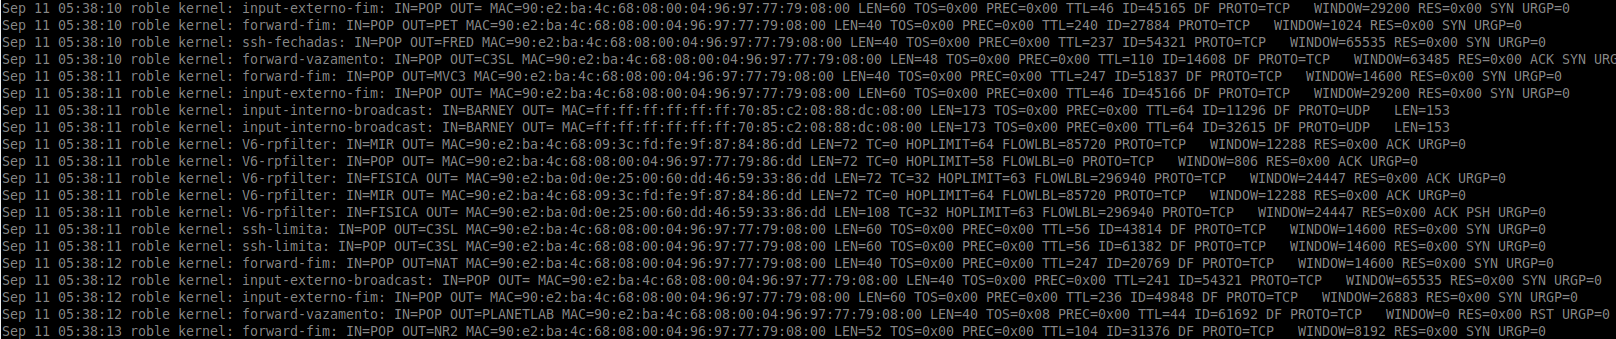
\includegraphics[width=\linewidth]{loglines.png}
		\caption{Exemplo de linhas do log}
		\label{fig:loglines}
	\end{figure}
	
	\pagebreak
	Todos os tipos de filtragem existentes se encontram em um arquivo "tipos-bloqueios", no formato:
	
	\begin{lstlisting}
	...
	V6-windows
	bios_debian
	bogon
	dns
	forward-fim
	forward-syn-piratas
	forward-vazamento
	input-externo-broadcast
	input-externo-fim
	...
	\end{lstlisting}
	
	O exercício consiste em fazer um script que retorne uma lista de tipos de bloqueios e suas ocorrências a partir de um log no formato descrito acima. A saída deve ser redirecionada para um arquivo contendo a data atual no nome. O script deve receber um parâmetro de versão. Versão V6, deve considerar todos os tipos de bloqueio que começam com "V6", versão "V4", deve considerar todos os tipos de bloqueios que \textbf{não} começam com "V6". Caso não receba nenhum argumento, todos os tipos de bloqueios devem ser considerados. O parâmetro de versão também deve ser identificado no nome do arquivo gerado. Os bloqueios sem nenhuma ocorrências devem aparecer no resultado. Caso um ou mais tipos de bloqueio tenham mais de 20000 ocorrências, o script deve enviar um e-mail com esses tipos de bloqueios e a quantidade de ocorrências de cada um deles.
	
	\pagebreak
	
	\section{Solução}
	
	\begin{lstlisting}
	1 #!/bin/bash
	2 
	3 # "Versão" sem o "-"
	4 ver=${1:1:2};
	5 # Organiza logs criados pela data e versão
	6 logn="log-$(date | awk -F " " '{print $3 $2 $6}')$ver";
	7 if [ -f $logn ]; then
	8     rm $logn;
	9     touch "$logn";
	10 fi
	11 
	12 if [ "$1" == "-V6" ]; then
	13     bloqTypes=$(grep "V6" tipos-bloqueios | tr "\n" " ");
	14 elif [ "$1" = "-V4" ]; then
	15     bloqTypes=$(grep "V6" -v tipos-bloqueios | tr "\n" " ");
	16 else
	17     bloqTypes=$(cat tipos-bloqueios | tr "\n" " ");
	18 fi
	19 
	20 mail=$(awk -v types="$bloqTypes" -v logn="$logn" '
	21 {countTypes[substr($6, 1, length($6)-1)] += 1}
	22 END {
	23     split(types, tps, " ");
	24     count = 1;
	25     for (tp in tps)
	26     {
	27         print tps[tp],":",(tps[tp] in countTypes) ? countTypes[tps[tp]] : 0 >> logn;
	28         if (countTypes[tps[tp]] > 20000)
	29         {
	30             print tps[tp], countTypes[tps[tp]];
	31         }
	32     }
	33 }
	34 ' log-firewall);
	35 
	36 echo "$mail" | mail -s "firewall warning $logn" "$USER"@inf.ufpr.br;
	\end{lstlisting}
	
	As linhas 3-10 servem para criar o log com o nome no formato: log-[data][versão]. Na linha 4, a variável \texttt{\textbf{\textit{ver}}} recebe o conteúdo dos índices 1 a 2 do primeiro parâmetro \texttt{\textbf{\textit{\$1}}}. Ou seja, removendo o índice 0, que contém o "-", restando apenas V6 ou V4. A data é obtida pelo comando "date", utilizando o awk para selecionar os campos necessários. Caso já exista um log com o nome gerado no diretório atual, ele é apagado, pois o resultado é inserido nesse arquivo linha por linha, com ">>", sem sobrescrever o conteúdo anterior.
	
	Nas linhas 12 a 18, os tipos de bloqueio são passados para a variável \texttt{\textbf{\textit{fileItemString}}} de acordo com a versão selecionada. A troca de \textbackslash n por espaços é necessária para que a cada elemento do array \texttt{\textbf{\textit{fileItemString}}} receba uma linha do resultado do grep.
	
	Na linha 20, o awk é invocado, com seu resultado sendo redirecionado à variável mail. Isso porque, dentro do awk, o real resultado será redirecionado ao arquivo criado no início do script, sendo assim, ainda é possível aproveitar o retorno do awk para retornar o conteúdo do email a ser enviado. São delclaradas 2 variáveis para o awk, contando os tipos a serem contados e nome do arquivo que deve receber o resultado.
	
	O fluxo principal do awk está na linha 21. Para cada linha, o array associativo \texttt{\textbf{\textit{countTypes}}}, é incrementado em cada índice. O índice é a substring da sexta coluna, removendo o último caractere, que em todos os casos é um ":". Note que não é necessário inicializar cada valor, dessa forma, ao final do arquivo, o array \texttt{\textbf{\textit{counTypes}}} contém todos os tipos de bloqueio como índice (incluíndo os tipos de bloqueio que não devem ser impressos no resultado, se houver), associados à quantidade de ocorrências de cada um deles.
	
	Ao final da execução principal do arquivo, no awk, nas linhas 22 a 33, para cada tipo de bloqueio (entre os bloqueios necessários para a versão escolhida), são impressos o índice associativo (tipo de bloqueio) da variável \texttt{\textbf{\textit{countTypes}}} e seu valor associado (quantidade de ocorrências) e se houverem mais de 20000 ocorrências desse tipo de bloqueio, esses valores são impressos ao retorno do awk (que no caso, é a variável mail).
	
	Na linha 36, um echo da variável \texttt{\textbf{\textit{\$mail}}} é usado como conteúdo do email, redirecionado ao comando mail. O campo assunto contém o nome do arquivo de retorno, que possui a data e versão da execução do script.
	
	\begin{figure}[h]
		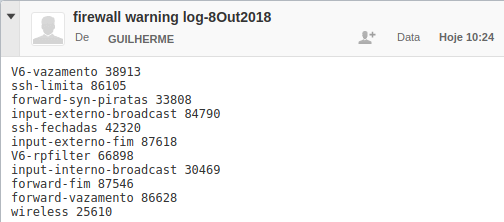
\includegraphics[width=\linewidth]{mail.png}
		\caption{Exemplo de Email enviado}
		\label{fig:mail}
	\end{figure}
	
	Para otimizar o desempenho, o script conta todos os tipos de bloqueio, independente de quais tipos de bloqueios serão impressos no resultado, assim, evitando branches no loop principal, que é na linha 21, onde o awk percorre cada linha do arquivo.
	
	\section{Conclusão}
	Como esperado, o bash não possui um menu gráfico com botões e opções de configuração, ao invés disso, o usuário pode configurar o bash através de variáveis pré-definidas e opções e realizar tarefas através de comandos. Além disso, o bash scripting não consiste apenas de variáveis e estruturas de controle do bash, e sim de um conjunto de comandos que, fazendo uso da árvore de diretórios e de redirecionamentos permitem ao usuário a automatização de tarefas que seriam exaustivas e repetitivas com uma interface gráfica. Dessa forma é possível dizer que o Bash não apenas facilita ou agiliza o uso do sistema e sim que ele expande as possibilidades do usuário. Após a leitura desse Tutorial, é ideal que cada usuário monte seu próprio ambiente de acordo com as suas necessidades (terminal, atalhos, aliases, configurações de bashrc, sistema operacional, editor de texto, etc...).
	
	
\bibliographystyle{apalike}
\bibliography{artbib}

%----------------------------------------------------------------------------------------
%   REFERENCE LIST
%----------------------------------------------------------------------------------------
\end{document}